\documentclass[a4paper,14pt]{extarticle}
\usepackage{../../tex-shared/report-layout}

\renewcommand{\mylabnumber}{1}
\renewcommand{\mylabtitle}{Исследование параметров и характеристик
симметричной проводной линии связи}
\renewcommand{\mysubject}{Инфокоммуникационные системы и сети}
\renewcommand{\mylecturer}{Чернега В.С.}

\begin{document}
\begin{titlepage}
    
    \thispagestyle{empty}
    
    \begin{center}
        
        Министерство науки и Высшего образования Российской Федерации \\
        Севастопольский государственный университет \\
        Кафедра ИС
        
        \vfill

        Отчет \\
        по лабораторной работе №\mylabnumber \\
        \enquote{\mylabtitle} \\
        по дисциплине \\
        \enquote{\MakeTextUppercase{\mysubject}}

    \end{center}

    \vspace{1cm}

    \noindent\hspace{7.5cm} Выполнил студент группы ИС/б-17-2-о \\
    \null\hspace{7.5cm} Горбенко К. Н. \\
    \null\hspace{7.5cm} Проверил \\
    \null\hspace{7.5cm} \mylecturer

    \vfill

    \begin{center}
        Севастополь \\
        \the\year{}
    \end{center}

\end{titlepage}

\section{Цель работы}
Изучение конструкции современных кабельных линий связи, используемых
в локальных компьютерных сетях, исследование методов измерения переходных
помех в симметричных линиях и степени искажений импульсов при передаче
данных по кабелям связи.

\section{Задание на работу}
\begin{enumerate}
    \item Изучить параметры и характеристики проводных и оптических линий связи.
    \item Создать модель симметричной двухпроводной линии связи в среде Proteus
          cо следующими параметрами:
          $C\text{\textit{п}} = 5 \text{ \textit{нФ/км},}$
          $L\text{\textit{п}} = 2 \text{ \textit{мГн/км},}$
          $R\text{\textit{п}} = 62\text{ \textit{Ом/км}.}$
    \item Запустить симуляцию заданной модели при использовании 2, 5 и 8 сегментов
          модели линии связи.
    \item Измерить амплитудно-частотную характеристику (АЧХ) и фазо-частотную
          характеристику (ФЧХ) для 1, 5 и 8 сегментов и полосу пропускания для
          различных длин сегментов.
    \item Оформить результаты в виде таблиц и графиков.
    \item Сделать выводы по работе.
    \item Составить отчет.
\end{enumerate}

\section{Ход работы}
Составим схему двухпроводной линии связи (\ref{fig:scheme}):
\begin{figure}[H]
    \centering
    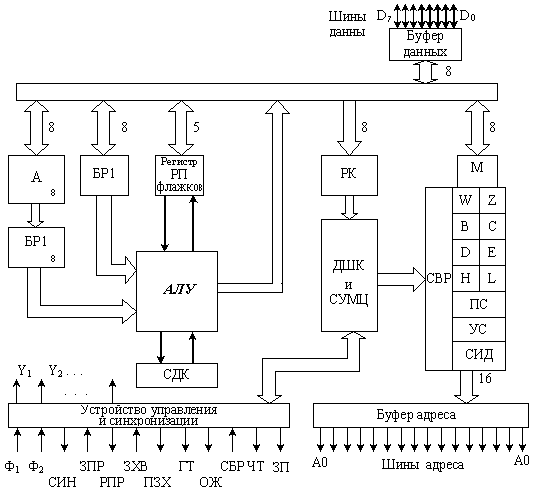
\includegraphics[width=\linewidth]{scheme}
    \caption{Схема двухпроводной линии связи}
    \label{fig:scheme}
\end{figure}

\end{document}